\begin{figure}

  \setlength{\unitlength}{\textwidth}
  \begin{picture}(1,0.3)(0,0.8)
    
    % % %90
      \put(0.025,0.9){\includegraphics[width=0.5\unitlength]{../FnP/gnuplot/lift_curve_165.eps}}
      \put(0.495,0.9){\includegraphics[width=0.5\unitlength]{../FnP/gnuplot/lift_curve_park.eps}}
     
   
	
            
      
      
   
 	\put(-0.01,1.02){ $c_y$} 	
% 	\put(0.56,1.02){ $\theta$}
 	
 	 	\put(0.25,0.88){ $\theta$} 	
 	 	\put(0.75,0.88){ $\theta$}



    \put(0.09,0.88){(a)}
    \put(0.56,0.88){(b)}
   
       

  \end{picture}

  \caption{Lift coefficient, $C_y$, as a function of incidence angle $\theta$, for a static square cross section at Re=165 by(a). Points ($\bullet$) are measurements from simulations.The data obtained by \cite{Parkinson1964} at Re=22300 are represented by (b). The solid line is a 7th-order polynomial fit that has been used to calculate the right-hand side of equation 4 throughout this study}
    \label{fig:lift_curves}
\end{figure}